\section{Core Problem}
\label{sec:core-problem}

In order to optimally schedule chunks over multiple connections we must differ between $2$ core problems:

\begin{itemize}
\item \term{Chunk Scheduling}
\item \term{Path Management}
\end{itemize}

When talking about \term{Chunk Scheduling} we mean making a decision for the next range $s$ to be requested over connection $c$. 
We will refer to the request range $s$ from now on as chunk size or chunk request, since the request range at the same time divides our web object into partial blocks of data. 

\begin{figure*}[t]
        \begin{minipage}[t]{0.5\linewidth}
		\begin{center}
                \subfigure[Bad Chunk Scheduling: Assuming $c_2$ has a higher throughput than $c_1$, here the better path has idle time due to bad scheduling towards the end of the file.]{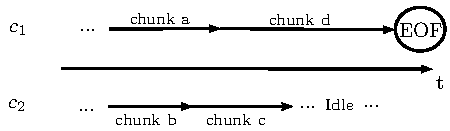
\includegraphics[width=\linewidth]{Figures/scheduler-why-1.pdf}}
        \end{center}
        \end{minipage}
~
        \begin{minipage}[t]{0.5\linewidth}
        \begin{center}
                \subfigure[Bad Path Management: Assuming $c_2$ has a higher throughput than $c_1$, here the better path has idle time due to a bad initial path choice.]{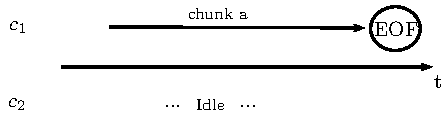
\includegraphics[width=\linewidth]{Figures/path-manager-why-1.pdf}}
        \end{center}
        \end{minipage}
        \caption{\label{fig:bad-scheduling} Illustration of bad chunk scheduling (a) and bad path choices (b).}
  \vspace*{-0.3cm}
\end{figure*}

\term{Path Management} refers to deciding which end-points to use for a new connections, \ie which client network interface and which server (IP) should connect.
Further, in case of website downloads we have to decide which paths we reuse. 
Choosing a bad performing path over a good performing one results in throughput loss and must be avoided. 
In~\xref{sec:path-management} we discuss in more detail our approaches for efficient \term{Path Management}.

In order to visualize the importance of solving these two problems, we illustrate cases of bad \term{Chunk Scheduling} and \term{Path Management} in~\fref{fig:bad-scheduling}. 

In~\fref{fig:bad-scheduling} (a) we illustrate how bad chunk scheduling can have a negative impact on the overall throughput. 
In this case a decision is made so that the slow connection $c_1$ starts downloading chunk $d$ which turns out to be the last block until EOF (end of file).
The decision is done while the fast connection $c_2$ still downloads chunk $c$ and this results in $c_2$ being idle for some time. 
A scenario like that might occur when the link throughput of $c_1$ drops unexpectedly while the assigned chunk size was too big, thus resulting in a much higher download time than expected. 
Especially in heavily used wireless environments rapidly time varying channel conditions are common and have to be taken into account.

Moreover, note that each HTTP request introduces an overhead consisting of a request and a response header, plus one round-trip-latency $rtl$ that is necessary to send the first request byte and receive the first response byte. 
Consequently, each chunk in \mhttp~introduces a request overhead. 
The overall goal of \term{Chunk Scheduling} is to have a minimum request overhead while still maintaining a certain adaptivity towards link changes. 
We see that being adaptive to link changes is of major importance since it is our goal to use each interface to its fullest throughput potential. 

Hence, for optimal \term{Chunk Scheduling} we have to keep two major key issues in mind:

\begin{itemize}
\item a small chunk size leads to higher link adaptivity, but at the same time increases the overall overhead
\item a big chunk size leads to less overhead, but at the same time reduces the overall link adaptivity
\end{itemize}

In~\fref{fig:bad-scheduling} (b) the impact of bad \term{Path Management} is illustrated. 
We see that in case of a small file, initially using the bad connection might lead to a scenario in which the good connection is never used and stays idle. 
This might especially occur in case of website downloads, since here many small files might be sequentially downloaded from the same domain. 
Hence, given we already used different paths and measured their performance, it is important to reuse the good over the bad performing ones. 
